\subsection{Image Processing}
%FERDIG
The digital camera is a powerful sensor that has many provides many advantages in technical applications and implementations. It is a sensor that can be used for the identification of environmental variables within the line of sight, and can easily be combined with other sensors. Many autonomous applications employ cameras, and together with image processing it provides a powerful tool to automate advanced tasks and real life objectives. Self-driving cars\cite{tesla} use cameras as well as other sensors to extract useful information from the environment.\\

As an example, in a self-driving car application, one might be interested in determining the size and location of other cars on the road in order to prevent collisions and provide an autonomous driving experience. Image processing is a topic that can be related to several fields of engineering, from simple automation to complex artificial intelligence.\\

In the following section I will present the fundamental underlying theory of edge detection and some of the image processing methods I use in my thesis.
%--------------

\subsubsection{Edge Detection}
%Omskrive litt
A powerful tool to use when trying to identify the characteristics of a the environment is edge detection. Edge detection is based on detecting sharp, local changes in intensity in an image. At a fundamental level, abrupt, local changes in intensity can be detected by using derivatives, where first- and second order derivatives are the most used \cite{g}. \\

Figure \ref{fig:derivatives} illustrates the differences between the intensity response of the first- and second order derivatives on an edge with a ramp response.

\begin{figure}[h]
  \centering
  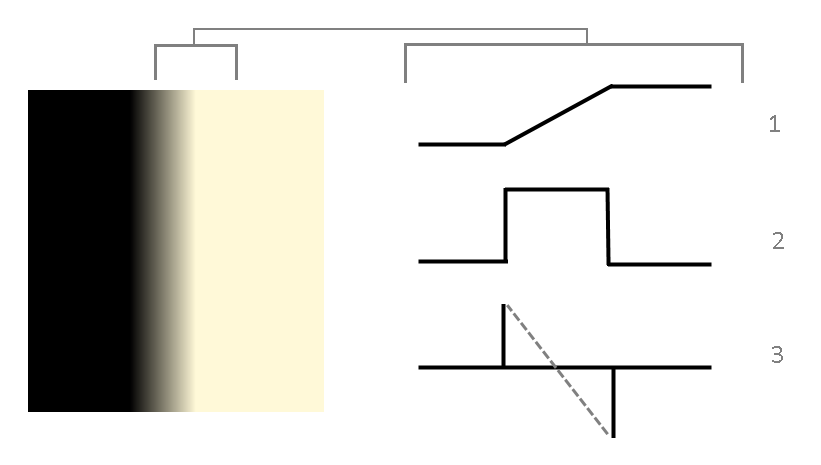
\includegraphics[width=0.8\textwidth]{fig/derivatives}
  \caption{(1) Horizontal intensity profile. (2) First derivative. (3) Second derivative with zero crossing}
  \label{fig:derivatives}
\end{figure}

\subsubsection{Edge Detection methods based on first derivatives}
%Omskrive litt
As mentioned previously, edges are characterized as a change in intensity in an image. Digital images are discrete, therefore we have to use an approximation of the first derivative with the requirements that; (1) it must be zero in areas of constant intensity, (2) it must be nonzero at the onset of an intensity step or ramp, and that (3) it must be nonzero at points along an intensity ramp\cite{g}. It is important to note that most edges in an image does not change its value immediately, but tends to change more gradually, like a ramp-function. Our requirements covers this, where the derivative must be non-zero along an intensity ramp.\\
We first consider the one-dimensional function $f(x)$, we approximate by Taylor expansion about $x$ of $f(x+\Delta x)$, where we let $\Delta x = 1$, and keep the linear terms:
\begin{align}
    \frac{\partial f}{\partial x} = f'(x) = f(x +1) - f(x)
\end{align}
We used the partial derivative here because the image is a function of two variables. We approximate the the derivative by Taylor expansion in the $y$ dimension just like we did above:
\begin{align}
\frac{\partial f(x,y)}{\partial x} = f(x+1,y)-f(x,y) = g_x\\
\frac{\partial f(x,y)}{\partial y} = f(x,y+1)-f(x,y) = g_y
\end{align}
A powerful tool in edge detection is to define the gradient, $\nabla f$ as
\begin{align}
\nabla f \equiv grad(f) \equiv 
\begin{bmatrix}
g_x \\
g_y
\end{bmatrix}
= 
\begin{bmatrix}
\frac{\partial f}{\partial x}\\
\frac{\partial f}{\partial y}
\end{bmatrix}\\
M(x,y) = \sqrt[]{g_x^2 +x_y^2}
\label{eq:magnitude}
\end{align}
Where the $\nabla f$ vector gives us information about the edge strength as well as the direction of the greatest rate of change of $f$ at location $(x,y)$.\\

The direction of the edge can be expressed as:
\begin{align}
\alpha(x,y) = \arctan(g_y/g_x)
\label{eq:direction}
\end{align}

Obtaining the gradient of an image involves calculation the partial derivatives $\frac{\partial f}{\partial x}$ and $\frac{\partial f}{\partial y}$ at every location of the pixels in the image. In order to do this we use spatial filtering in the image (also known as masking). The process of spatial filtering consists of moving a filter mask from point to point in an image, and calculating the filter response of the original image at each point $(x,y)$ in the image. The filter values are pre-defined and characteristics of the filter can be modified in order to achieve different improvements in an image such as image enhancement.\\

We want to look for edges in two dimensions; x and y direction, thus the most used edge detection algorithms use 2D spatial filters to find edges. A general 3x3 spatial filter mask can be represented as a table of intensity values $z_i$ as illustrated in Table \ref{spatial}.
\begin{table}[h]
\centering
\caption{General 3x3 Spatial Filter Mask}
\label{spatial}
\begin{tabular}{|l|l|l|}
\hline
$z_1$ & $z_2$ & $z_3$\\ \hline
$z_4$ & $z_5$ & $z_6$\\ \hline
$z_7$ & $z_8$ & $z_9$\\ \hline
\end{tabular}
\end{table}

Edge detection methods based on the first derivative are generally more primitive than those based on the second order derivative. They are generally less computationally intensive, but offer limited functionality and robustness. For my application I will implement a method based on the second derivative.

\subsubsection{Edge Detection methods based on the second derivative}
%Skrive om at det er dette vi bruker i vår applikasjon
The requirements set on the approximation of the second order derivative is similar to that set on the first order derivative. The only difference is that I now only require the second order derivative to be non-zero at the onset and end of a ramp in intensity value. This means that the first order derivative methods will create "thicker" edges since its non-zero along the whole ramp, while the second order derivative methods will lead to "thinner" edges, since the values are non-zero only at the beginning and the end of a ramp.



\subsubsection{Canny edge detection method}
%endre litt, ikke "a different edge detection alg---"
A complex edge detection algorithm is the Canny edge detector\cite{canny}. In general, the Canny method is regarded as superior to most other edge detection algorithms, including other edge detector based on the second derivative, and is based on three objectives:
\begin{itemize}
\item Low error rate. The algorithm should find all the edges in an image, regardless or orientation. Should be as close as possible to the actual edges.
\item Edge points should be well localized. Detected edges should be close to the actual edges.
\item Single edge point response. Should not return multiple edge points where only a single edge point exist.
\end{itemize}
The Canny method starts with applying a Gaussian filter to convolve with the image in order to smooth out noise. After this the gradient magnitude (\ref{eq:magnitude}) and the direction (\ref{eq:direction}) are calculated:
\begin{align*}
M(x,y) = \sqrt[]{g_x^2 +x_y^2}\\
\alpha(x,y) = \arctan(g_y/g_x)
\end{align*}
After this it applies a non-maximum suppression technique to the gradient magnitude image which thins the edges. This helps suppress all the gradient values to zero except the local maximal, which is the the sharpest change in intensity value, thus fulfilling the objective of giving a single edge point response.\\

The last part of the algorithm is to use double thresholding to determine strong and weak edges. Edges with intensity values below the lowest threshold are suppressed, which is noise in most cases. This is a tuning parameter and needs to be determined empirically. The last step of the algorithm also involves tracking edges and conducting a connectivity analysis to detect and link edges together, where edges that are weak and not connected to strong edges are suppressed.\\

\newpage
%Skal jeg ha med dette?
\subsection{Image pre-processing before Edge detection}
There are a number of different techniques and methods one can employ before using an edge detection algorithm to get a better edge detection result.
\subsubsection{Correcting Nonuniform Illumination}
Depending on the lighting conditions in the image, it might be beneficial to correct for nonuniform illumination. This can be done in several ways, but the most normal being estimate the background illumination of the image, inverse it and subtract it from the original image.
\subsubsection{Smoothing}
Smoothing is beneficial to suppress noise in the image. This can be done by applying a Gaussian filter to the image, which described previously in some of the edge detection algorithms. Smoothing is a part of some of the edge detection algorithms, which is designed to suppress noise.
\subsubsection{Increase contrast}
Increasing contrast can help in the detection of edges in an image. This is done by saturating the top and bottom $1\%$ of intensity values in the image. In the implementation described later in the report, this is utilized to improve the edge detection algorithm.
\subsubsection{Re-sizing}
By re-sizing the image by a scale factor the image will be smoothed. Some edge detection algorithms work better with images that are scaled down and smoothed. This is described later in Section \ref{testing}, and how this affects edge detection and edge linking quality.
%-----------

\newpage
\subsection{Edge Linking}
%Skrive slik som vi gjør det i OpenCV
After the edge detection algorithm has been applied to the image, we ideally have detected all the edge pixels in the image perfectly. Most of the time, this is not the case. The edge detection is therefore followed up by edge linking, where we attempt to assemble edge pixels into meaningful edge segments. Since actual edges will have the property of being fully or partly connected straight lines, noise in the image will naturally be suppressed and not detected. 
%--------

\subsubsection{Hough Transform}\label{ch:hough}
%Skrive slik jeg gjør i opencv
The Hough transform is a global processing method of edge linking \cite{hough}.  Considering a point $(x_i,y_i)$ in the xy-plane, we can describe infinitely many lines running through this point as $y_i = ax_i + b$ for any $a$ and $b$. We can rewrite this as $b = -ax_i + y_i$, and consider the ab-plane, which is known as the parameter space. This gives an equation for a single line for a single xy-pair $(x_i,y_i)$. A different xy-pair $(x_j,y_j)$ also has a line expressed in parameter space $b = -ax_j + y_j$, and if the lines are not parallel, the lines will intersect at a point $(a',b')$. $a'$ is the slope, and $b'$ is the intercept of the line containing both $(x_i,y_i)$ and $(x_j,y_j)$. The points on this line will have lines in the ab-plane that intersects at $(a',b')$.\\

One fundamental problem representing lines on the form $y = ax + b$ is that $a$ approaches infinity as the line gets closer to vertical. It is therefore beneficial to represent the lines as:
\begin{align*}
x\cos{\theta} + y\sin{\theta} = \rho
\end{align*}
This is a transformation to the $\theta\rho$-plane, which is very similar to that of the ab-plane. $(\theta',\rho')$ corresponds to the line that passes through both $(x_i,y_i)$ and $(x_j,y_j)$. When $(\theta',\rho')$ has a high concentration of curves passing through it, it indicates that these curves are a part of a connected line in the xy-plane. The Hough transform algorithm can be expressed as\cite{g}:
\begin{enumerate}
\item Use edge detection on an image and obtain a binary image edge image
\item Transform image to the $\theta\rho$-plane
\item Count and examine lines intersecting in the $\theta\rho$-plane
\item Determine the lines based on number of intersects in $(\theta',\rho')$
\end{enumerate}
By using Hough transform the length of each wall segment can be extracted in pixel values. This is very important to make us able to map the maze in real-life units.
%-----------

\subsection{Mapping}
\label{ch:mapping}
The primary goal in this project is to be able to map a maze. Techniques explained previously lays the ground work for how we are able to extract useful information from the image to be used for mapping. In addition to the information extracted by the image, we need some additional information for mapping:
\begin{itemize}
\item Height $H_{tot}$ above ground the image was taken from as well as x-y position
\item The orientation of the image sensor
\item Assume we know the height of the walls $H_w$
\item Information about the image sensor (pixel pitch $p$ and focal length $f$)
\end{itemize}
We also put the following assumptions on the maze and image:
\begin{itemize}
\item The wall height $H_w$ is constant on the entire maze
\item The walls are straight (no curves)
\item The walls are normal to the ground (no angle)
\item The line of sight of the image covers the entire maze (one image sufficient)
\end{itemize}
Figure \ref{fig:mapping} displays the setup and different heights and planes associated with our mapping looking perpendicular to the ground. We can see that the wall plane height $H_p = H_{tot} - H_w$. 
\begin{figure}[H]
\centering
\includegraphics[width=\linewidth]{fig/Mappingsetup}
  \caption{Mapping setup}
  \label{fig:mapping}
\end{figure}
One key insight in this setup is a result of taking the image normal to the ground and wall plane. Looking at Figure \ref{fig:mapping}, we can see that if we used the total height $H_{tot}$ in our calculation, the top of the wall would be projected an error $e$ away from the actual base of the maze. Since we are taking the image normal to the ground, and we know the height of the wall $H_w$, we can move to the wall plane and do our calculations here instead of doing it at the ground plane, thus eliminating the error $e$. We can simply move our projected map a distance $z = -H_w$ after the mapping is done to coincide the top of the wall with the base of the wall.

\subsubsection{Determining the length of the walls}
As mentioned previously, Hough transform gives us the straight line segments of the maze and their respective lengths in pixels are easy to extract. The Hough transform algorithm outputs a list of x-y coordinates in pixels that define the start- and end-point of each detected line segment. To extract the lengths of each line segment we can use:
\begin{align}
\textbf{Length of line} = l_i = \sqrt{(x_{i+1} - x_i)^2 + (y_{i+1} - y_i)^2 }\quad [pixels]
\end{align}
Ground Sample Distance (GSD) can now be used to convert these lengths in pixels to lengths in meters. The length $L$ can be expressed in [m]:
\begin{align}
L_i = l_i \times GSD\quad [m]\\
L_i = l_i \times \frac{p}{fW}H_p\quad [m]
\end{align}
Where $H_p$ is the distance from the optics to the top of the wall and $W$ is the width of the image in pixels. $p$ is the pixel pitch and $f$ is the focal length of the image sensor.  

\subsubsection{Determining the position of the walls}
The information used when finding the length of the walls can be also used to transform the position in the image to their respective real-life position. The Hough transform outputs a list of the start and end position of the line segments in pixels. To transform these values to real life values we need information about the location of the image sensor. When taking the image, we assume we have measurements for the x-y position in the real world of the image sensor. Since we are taking the picture normal to the wall- and ground plane, the x-y position of the image sensor in the real world corresponds to the center of the image.\\

There are several ways to extract and transform the position of the walls from the Hough transform to real-life units. One way is to transform the start- and end point coordinates in pixels of each wall segment to meters with respect to the image center. This can be done by first finding the GSD of the image and after that subtracting the x- and y component of each start- and end point by the x- and y component of the center and multiplying by the GSD.\\

If we have the position of the center $(x_c,y_c)$ and the start- and end point of a line segment $(x_1,y_1)$ and $(x_2,y_2)$ in the image respectively. The position of each of these points relative to the center can be expressed as:
\begin{align}
\textbf{Position of start point} = GSD\times(x_1-x_c, y_1-y_c)\quad [m]\\
\textbf{Position of end point} = GSD\times(x_2-x_c, y_2-y_c)\quad [m]
\end{align}
Since we know the start and end point coordinates in real life units of all wall segments, we have all the information we need to express the characterization of the maze. We assume we know the orientation of the image sensor when the image is taken, giving us a complete characterization of where each wall segment is in the real world. \\

It is important to note that I am not calculating or implementing the orientation of the image sensor when the image is taken. It is assumed we have a measurement of the orientation about an inertial axis in the ground- and wall plane, so that the mapping directly relates to this inertial frame. This means that we require the UAV to measure the attitude when mapping the maze.




















